\chapter{ \textit{Lustre} }
\section{Увод}

\textit{Lustre}   систем је бесплатан, дистрибуиран, паралелни фајл систем развијен од стране \textit{Sun Microsystems Inc}.  \textit{Lustre}  систем је дизајниран и имплементиран тако да смањи  или потпуно неутралише уска грла пређашњих паралелних фајл система. Централна компонента   \textit{Lustre}  система је дељени фајл систем за кластере.  \textit{Lustre}  је тренутно доступан за Linux оперативне системе и омогућава \textbf{UNIX®} фајл систем окружење.  \textit{Lustre}  архитектура се користи за више врста кластера. Користи се у седам од десет највећих кластера високих перфоманси у свету који имају хиљаде клијента, петабајте складишта и хиљаде  гигабајта у секунди У/И операција. Скалабилност коју нуди   \textit{Lustre}  учинила га је погодним алатом у оквиру истраживања нафте и гаса, у производњи као и у финансијском сектору. Са корисним побољшањима подршци у оквиру  \textit{Lustre}  мреже (\textit{LNET}) и софтверима који управљају  \textit{Lustre}  фајл системом, коришћење  \textit{Lustre}  фајл система би требало да буде још шире. Скалабилност   \textit{Lustre}  система смањује потребу за одвојеним фајл системима, на пример креирање једног фајл система за један кластер или још неефикасније један фајл систем за сваки \gls{NFS} фајл сервер. Ово доводи до предности управљања складиштем података, избегавајући вишеструке копије података на више фајл система. Главни  \gls{HPC} центри због тога захтевају много мање складишта података са   \textit{Lustre}  фајл системом него са другим системима. Проток или капацитет може се лако подесити после инсталације кластера, уколико се дода нови сервер. Како је   \textit{Lustre}  бесплатан систем, усвојен је од стране једног броја рачунарских компанија и интегрисан је њиховим понудама. У циљу једноставне инсталације   \textit{Lustre}  фајл система, \textit{Red Hat} и \textit{Novell} (\textit{SUSE}) нуде закрпе кернела својих дистрибуција.  \textit{Lustre}  архитектура први пут је развијена 1999. године, а 2003. године је објављена верзија 1.0 и одмах је искоришћена на великом броју кластера високих перформанси. Коришћење   \textit{Lustre}  система такође је утицало и на побољшање перформанси \textit{Linux ext3} фајл система.


\newpage
\section{Компоненте  \textit{Lustre}  фајл система}
\subsection{Основне компоненте}
\textit{Lustre} фајл систем се састоји од следећих основних компоненти(слика 2.1):
\begin{itemize}
\item
\textbf{Management Server(MGS)} 
 Чувa информације o конфигурацијама за све \textit{Lustre} системе у кластерy. Сваки \textit{Lustre} клијент контактира MGS да пружи информације. MGS захтева сопствени диск за складиштење. Међутим, постоји одредба која омогућава дељење MGS дискa (\zn ко-лоцирање") са једним MDT-ом. MGS се не сматра \zn делом" индивидуалног фајл система, већ пружа информације о конфигурацији за \textit{Lustre} компоненте.
 
\item 
\textbf{Metadata Server (\gls{MDS})} 
 MDS сервер чине метаподаци ускладиштени у један или више MDT сервера који су на располагању \textit{Lustre} клијентима. Сваки MDS  управља именима фајлова и директоријумима \textit{Lustre} система и обезбеђује мрежни захтев за руковање једним или више локалних MDT-а.

\item 
\textbf{Metadata Target (\gls{MDT})} 
 MDT чувa метаподатаке (као што су имена фајлова, директоријума, дозвола и распоред фајлова) на MDS-у. Сваки фајл систем има по један MDT. MDT на дељивом фајл систему може бити доступан многим MDS серверима, мада само један заправо треба да га користи. Уколико дође до грешке на MDT-у, MDS може аутоматски преузети његову улогу и ставити се на располагање клијентима. Ова могућност се назива MDS \textit{ failover}.

\item 
\textbf{Object Storage Servers (\gls{OSS})} 
 OSS обезбеђују улазно/излазне операције, као и захтеве за један или више локалних OST-а. Обично OSS опслужује између 2 и 8 OST-а, од којих један OST може имати до 16 TB складишног простора.  MDT, OST и \textit{Lustre} клијенти могу се покренути истовремено на једном чвору. Међутим, најзаступљенија конфигурација је да се MDT инсталира на одвојеном чвору, са једним или више OST-а на сваком OSS чвору.

\item 
\textbf{Object Storage Target (\gls{OST})} 
 OST чува податке (делове корисничних фајлова) на једном или више OSS-а. Један \textit{Lustre} фајл систем може имати више OST-а, од којих сваки опслужује део фајла. Није нужно да се један фајл налази на једном OST-у. У циљу оптимизације перформанси, фајл може бити расподељен на много OST-а. Logical Object Volume (LOV) управља деловима датотека на вишеструким OST.

\item 
\textbf{Lustre клијенти} 
 Lustre клијенти су рачунари који по покретању \textit{Lustre} програма омогућавају подизање партиције \textit{Lustre} система. \textit{Lustre} програм се састоји од окружења између \textit{Linux Virtul File System-a} и \textit{Lustre} сервера. Сваки клијент се састоји од: \textit{Metadata Client (\gls{MDC})}, \textit{Object Storage Client (\gls{OSC})} и \textit{Management Client (\gls{MGC})}. Група OSC се налази у једном LOV. Радећи здружено, OSC  омогућава  транспарентан приступ фајл систему. Клијенти који подижу \textit{Lustre} фајл систем виде један кохерентан и синхронизован фајл систем све време. Различити клијенти могу да уписују различите делове истoг фајла истовремено, док остали клијенти могу да читају из фајла.
\end{itemize}

\subsection{\textit{Lustre} Умрежавање (\gls{LNET})}

Lustre умрежавање (LNET) је \textit{\gls{API}} који управља мета подацима и улазно/излазним податацима за системске сервере и клијенте. LNET подржава више хетерогених окружења на клијентима и серверима. LNET комуницира са више врста мрежа преко \textit{Network Abstraction Layers (\gls{NAL})}. Lustre систему су на располагању већи број мрежа, укључујући \textit{Infiniband}, \textit{TCP/IP}, \textit{Qуadrics Elan}, \textit{Myrinet (MX and GM)} и \textit{Cray}.  Код кластера са \textit{Lustre} системом, сервери и клијенти комуницирају са дрyгом врстом мреже која се зове \textit{Lustre Networking (LNET)}, док су складишта MDS and OSS повезана традиционалним SAN технологијама.

\paragraph*{Кључне карактеристике \textit{Lustre} мреже}
\begin{itemize}
\item
RDMA - подршка мрежа као што су \textit{Elan}, \textit{Myrinet} и \textit{InfiniBand}.

\item
Подршка за много чешће коришћене типове мрежа попут \textit{InfiniBand} и \textit{TCP/IP}.

\item
Својства висока доступности и опоравка омогућавају транспарентан опоравак сервера.

\item
Истовремена доступност више мрежних типова са рутирањем између њих.
\end{itemize}

\begin{figure}[h!]
  \centering
      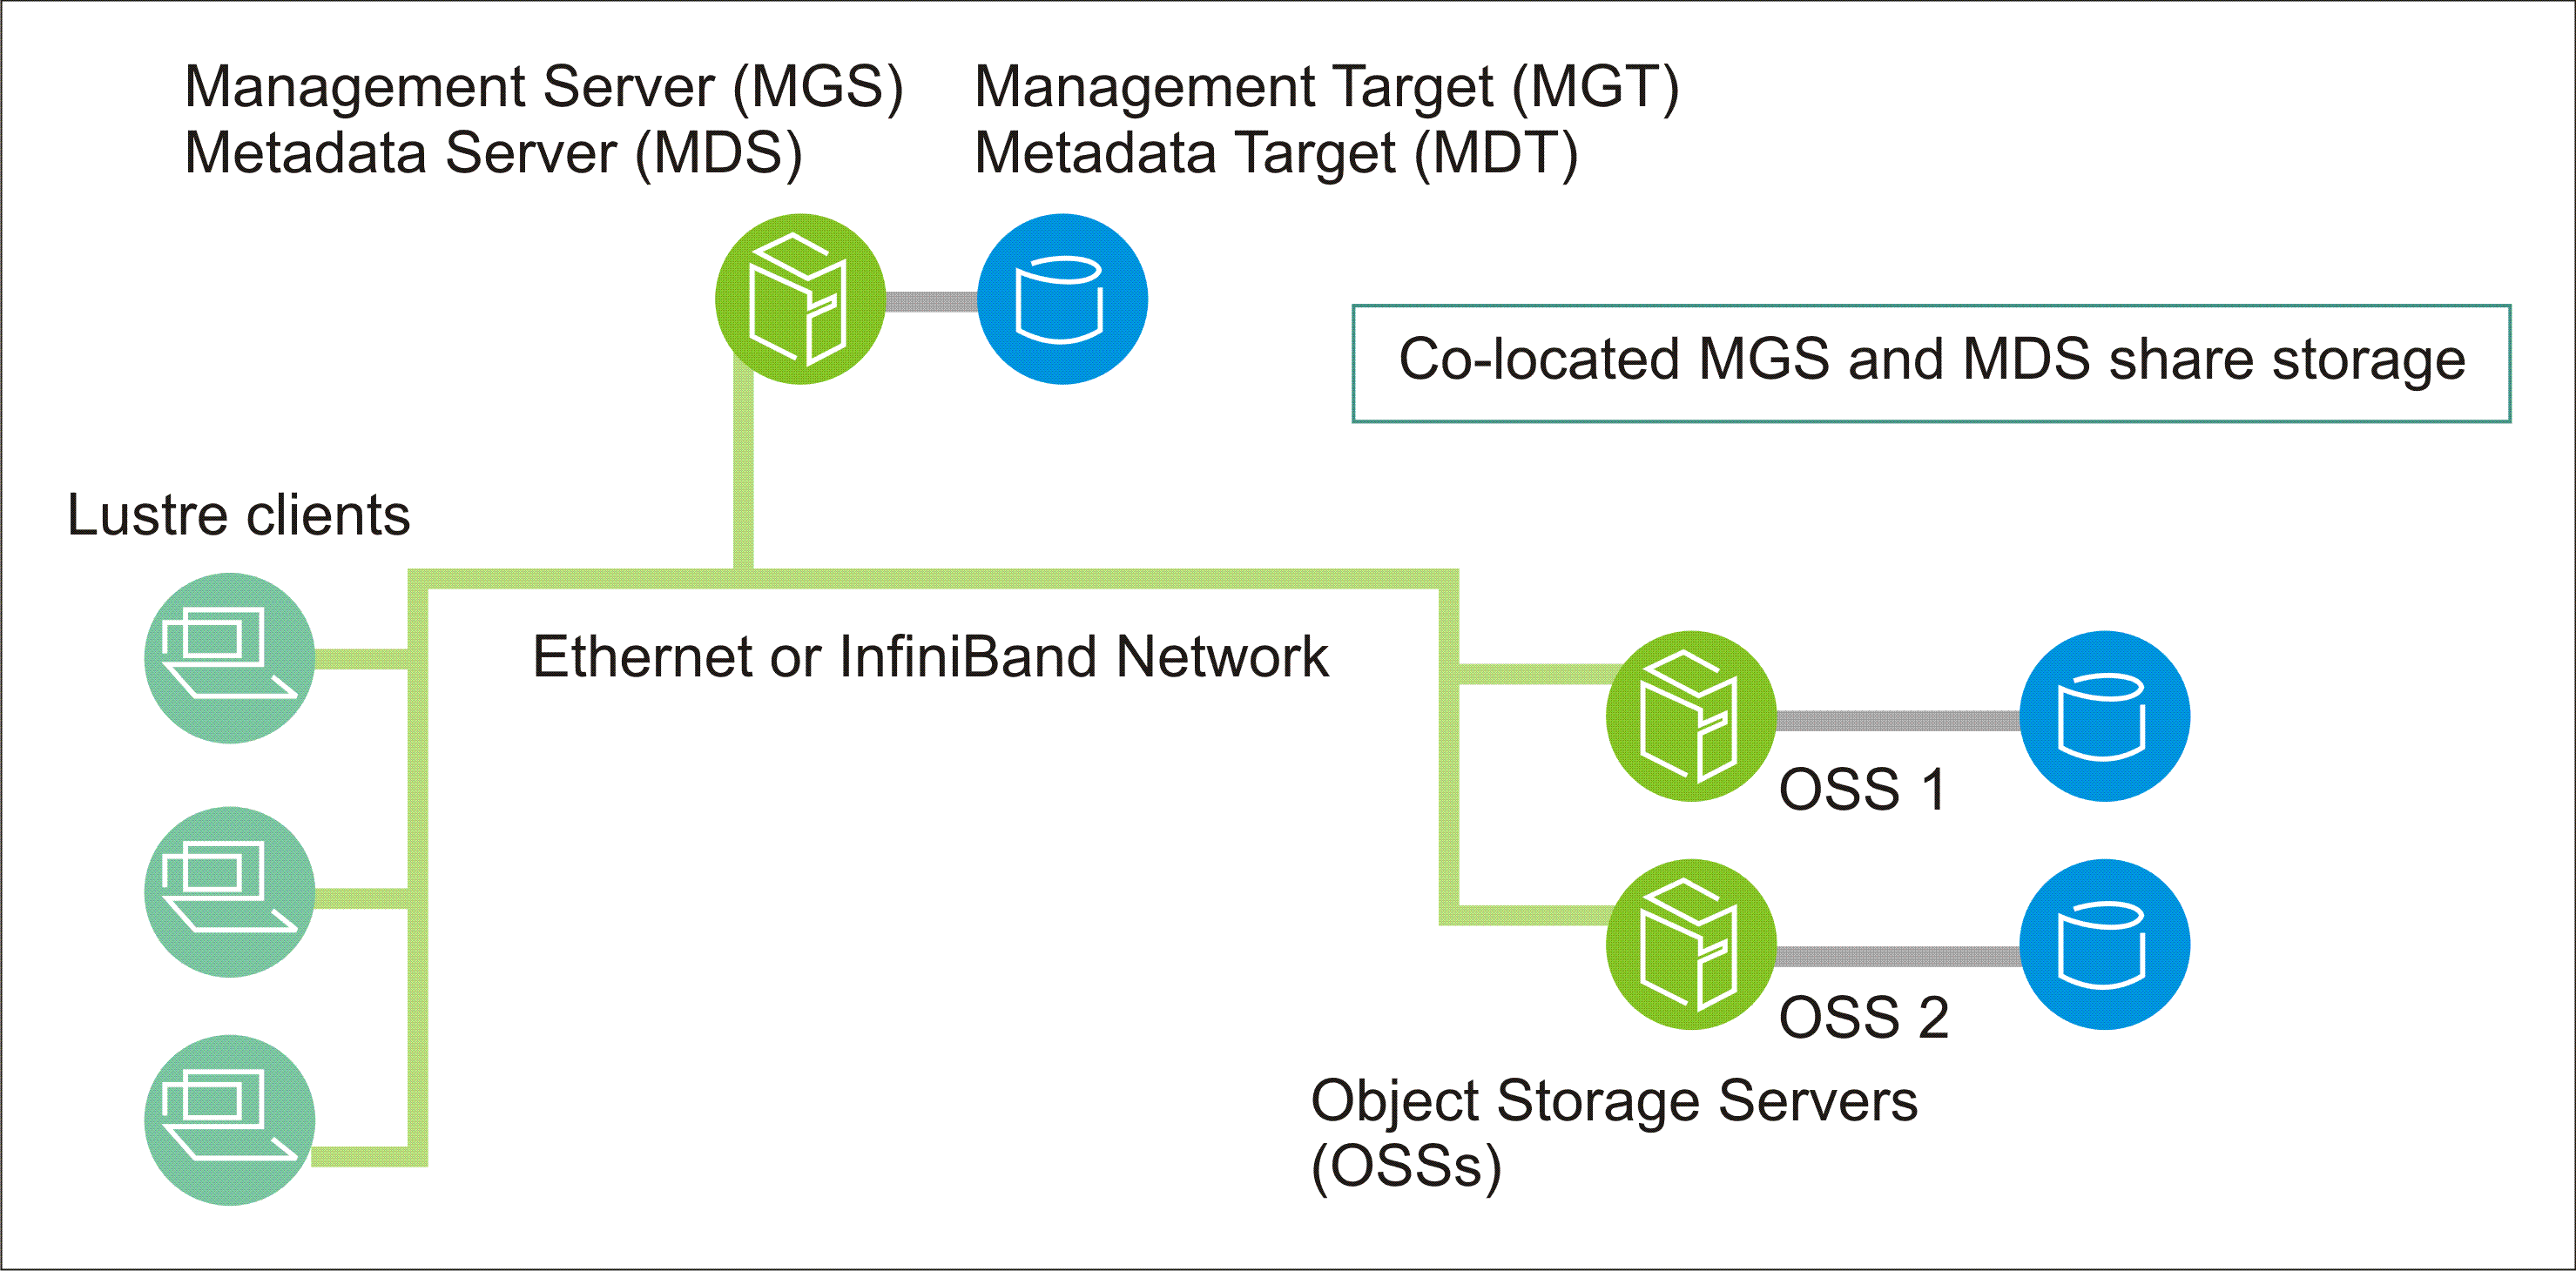
\includegraphics[width=1\textwidth]{slike/lustre.png}
  \caption{\textit{Lustre} компоненте}
\end{figure}



